In this section we provide mockups of a possible UI for our room draw website.

\subsection{Main Pages}
\subsubsection{Login Page}

\begin{figure} \centering

\includegraphics[scale=.15]{wireframe/login}
\caption{a login page}
\label{fig:wirelogin}
\end{figure}

We begin perhaps unsuprsingly with a simple login page (\cref{fig:wirelogin}).
At minimum, this page should allow a student with a valid username and password
to proceed to the sites that follow, populating those sites with the correct
information as matching to the student's username. It should also reject a
invalid logins.

As a possible extension, this page may support adminstrator logins. In which
case, an admin might have different acess and a stronger ability to make
changes.

A successful login should result in being passed to an interface similar to
those that follow, though perhaps without any of the leftmost boxes selected.

\subsubsection{Map page}

\begin{figure} \centering
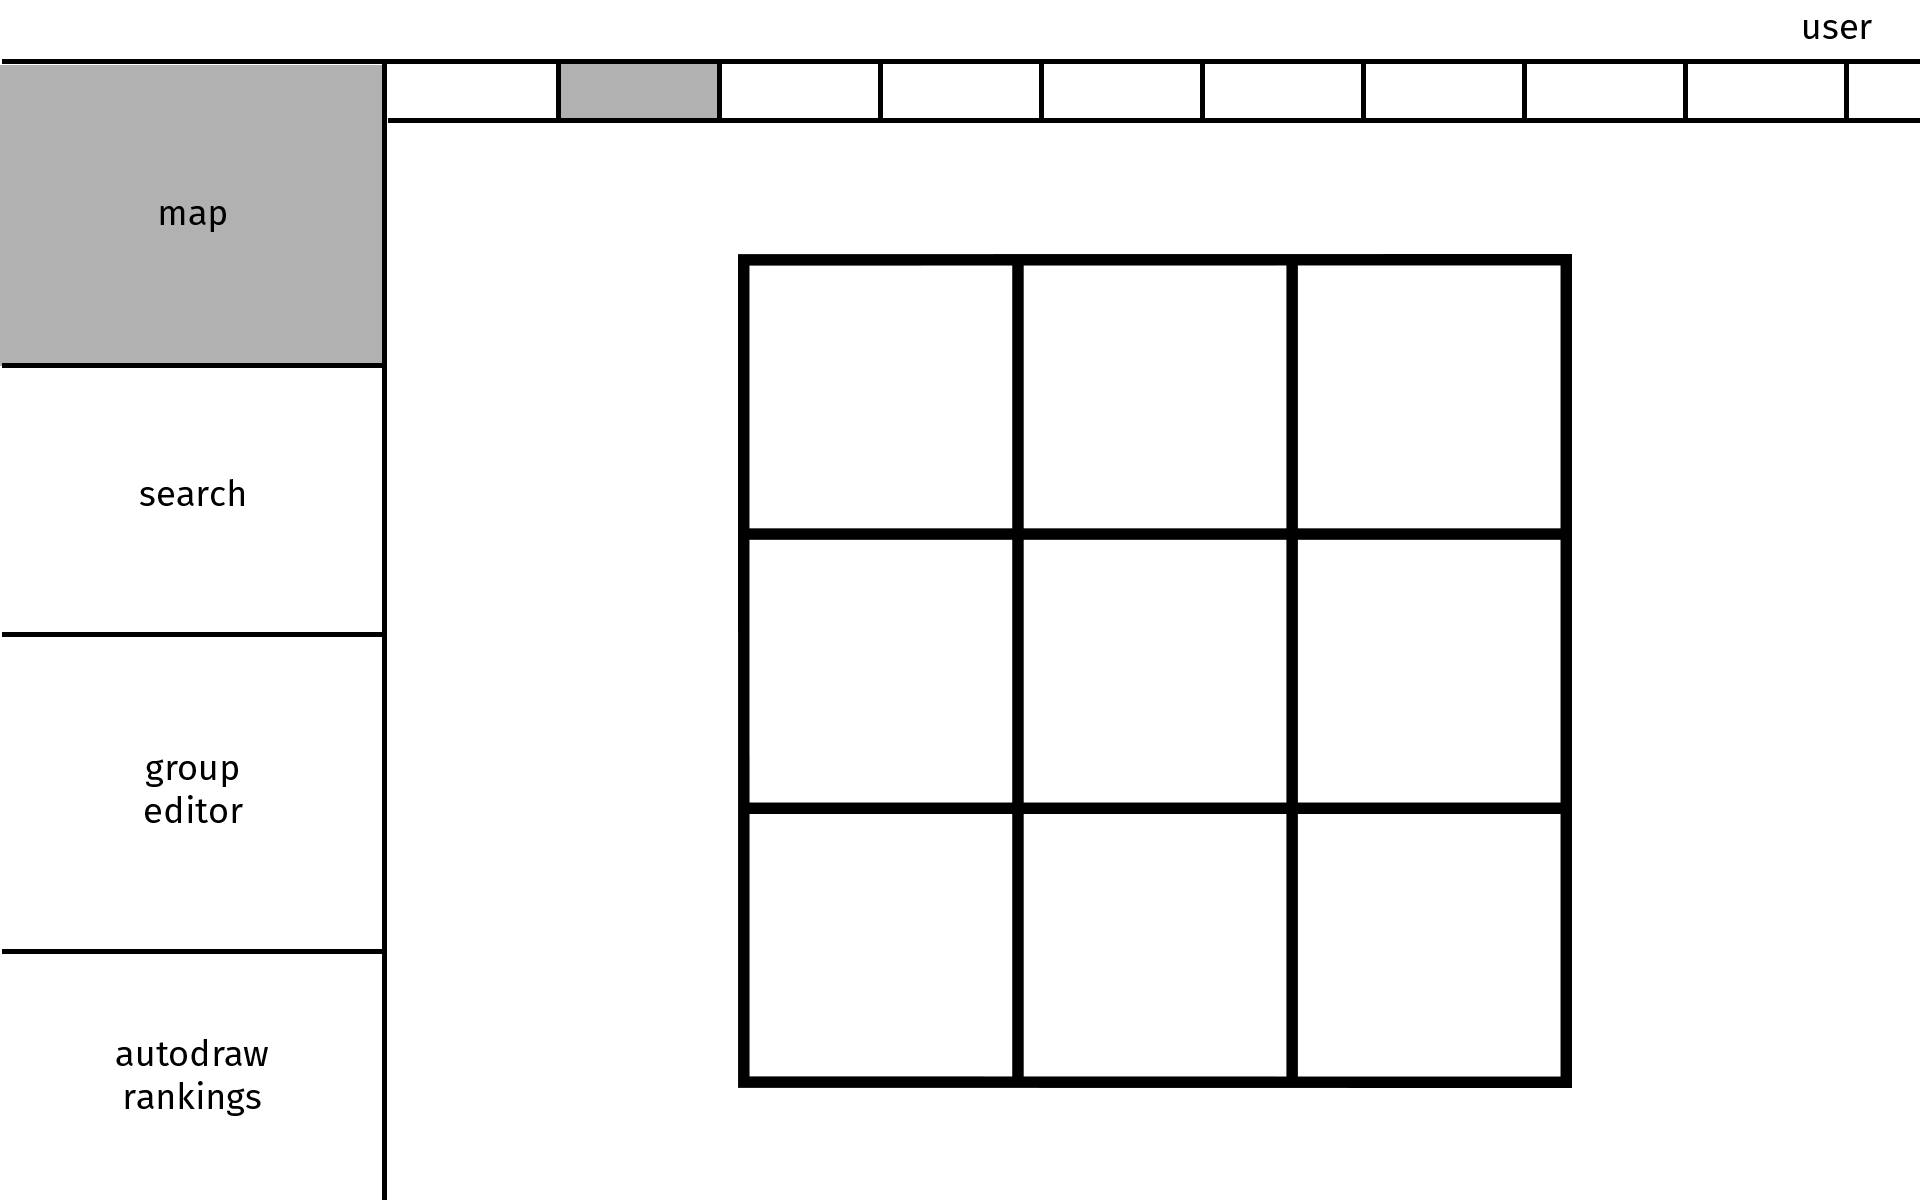
\includegraphics[scale=.15]{wireframe/map}
\caption{a page to see dorm maps}
\label{fig:wiremap}
\end{figure}

The first page selector leads to the ``Map'' page as seen in \cref{fig:wiremap}.
Across the top of the main frame of this page, one can expect to see a listing
of the various dorms on campus. Each of these listed dorms may be thought of as
a clickable tab. Upon a click, the corresponding map(s) for that dorm will fill
up the main section of the page.

A possible extension, though one we consider well beyond the scope of the
project as we image it, could be to enable click-actions on the maps. By this we
mean that if a particular dorm is clicked on the map, a context menu could
appear, offering the user to add the selected dorm (or suite) to their autodraw
queue.


\subsubsection{Search Page}
\begin{figure} \centering
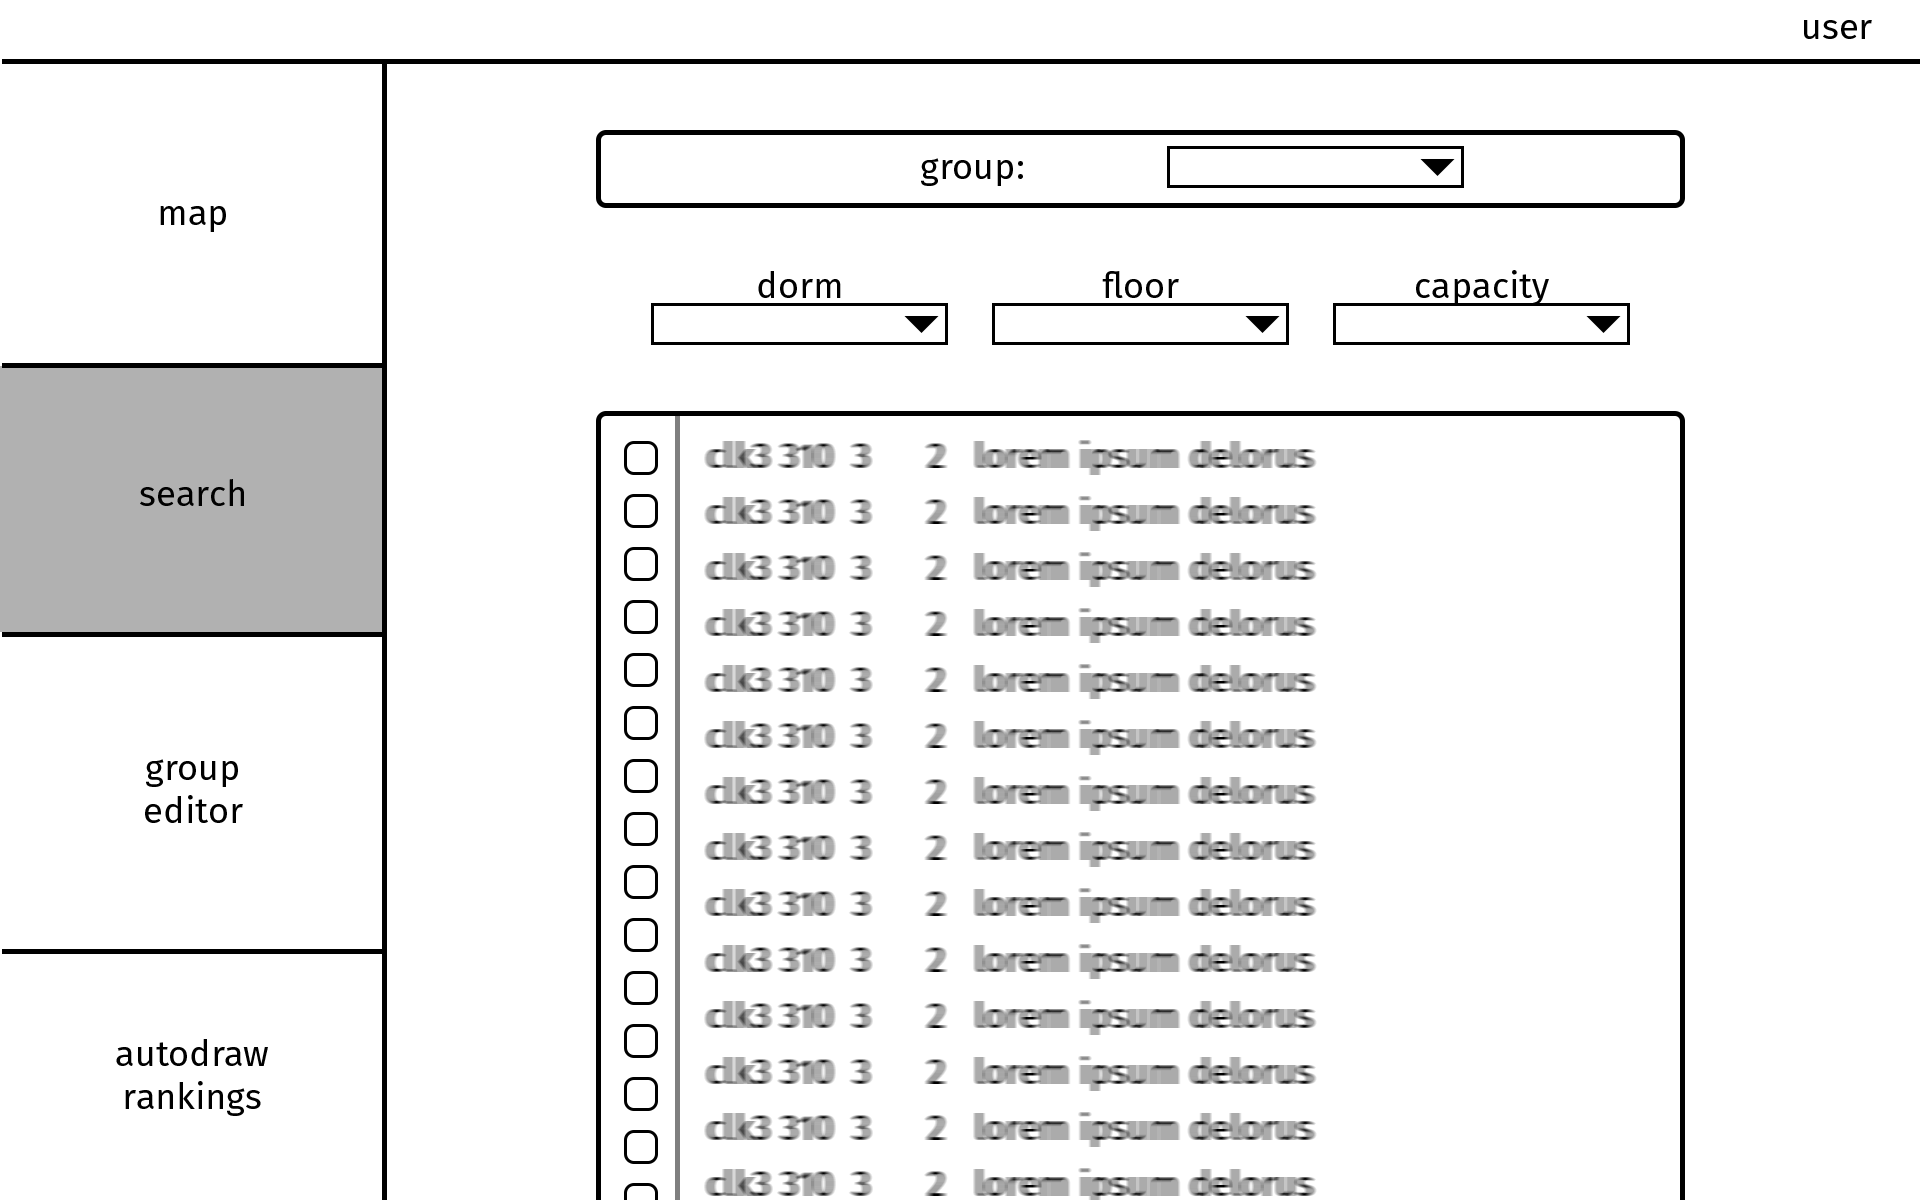
\includegraphics[scale=.15]{wireframe/search}
\caption{a page to filter through dorm listings and add them to one's queue}
\label{fig:wiresearch}
\end{figure}

The second choice on the left bar loads the ``Search'' page as seen in
\cref{fig:wiresearch}. On this page, a user may select the group for which
they're searching and may filter through the dorms. These filters may include
options like dorm name, floor, capacity, available, sqft, suite, etc.

The checkboxes that appear beside each result behave as follows. Checking an
unchecked box will add the corresponding room/collection to the autodraw
preference queue. Prechecked boxes indicate that the room/collection is already
present on the selected group's autodraw queue. Unchecking a currently checked
box will remove that room/collection from the selected group's autodraw queue.


\subsubsection{Group Page}
\begin{figure} \centering
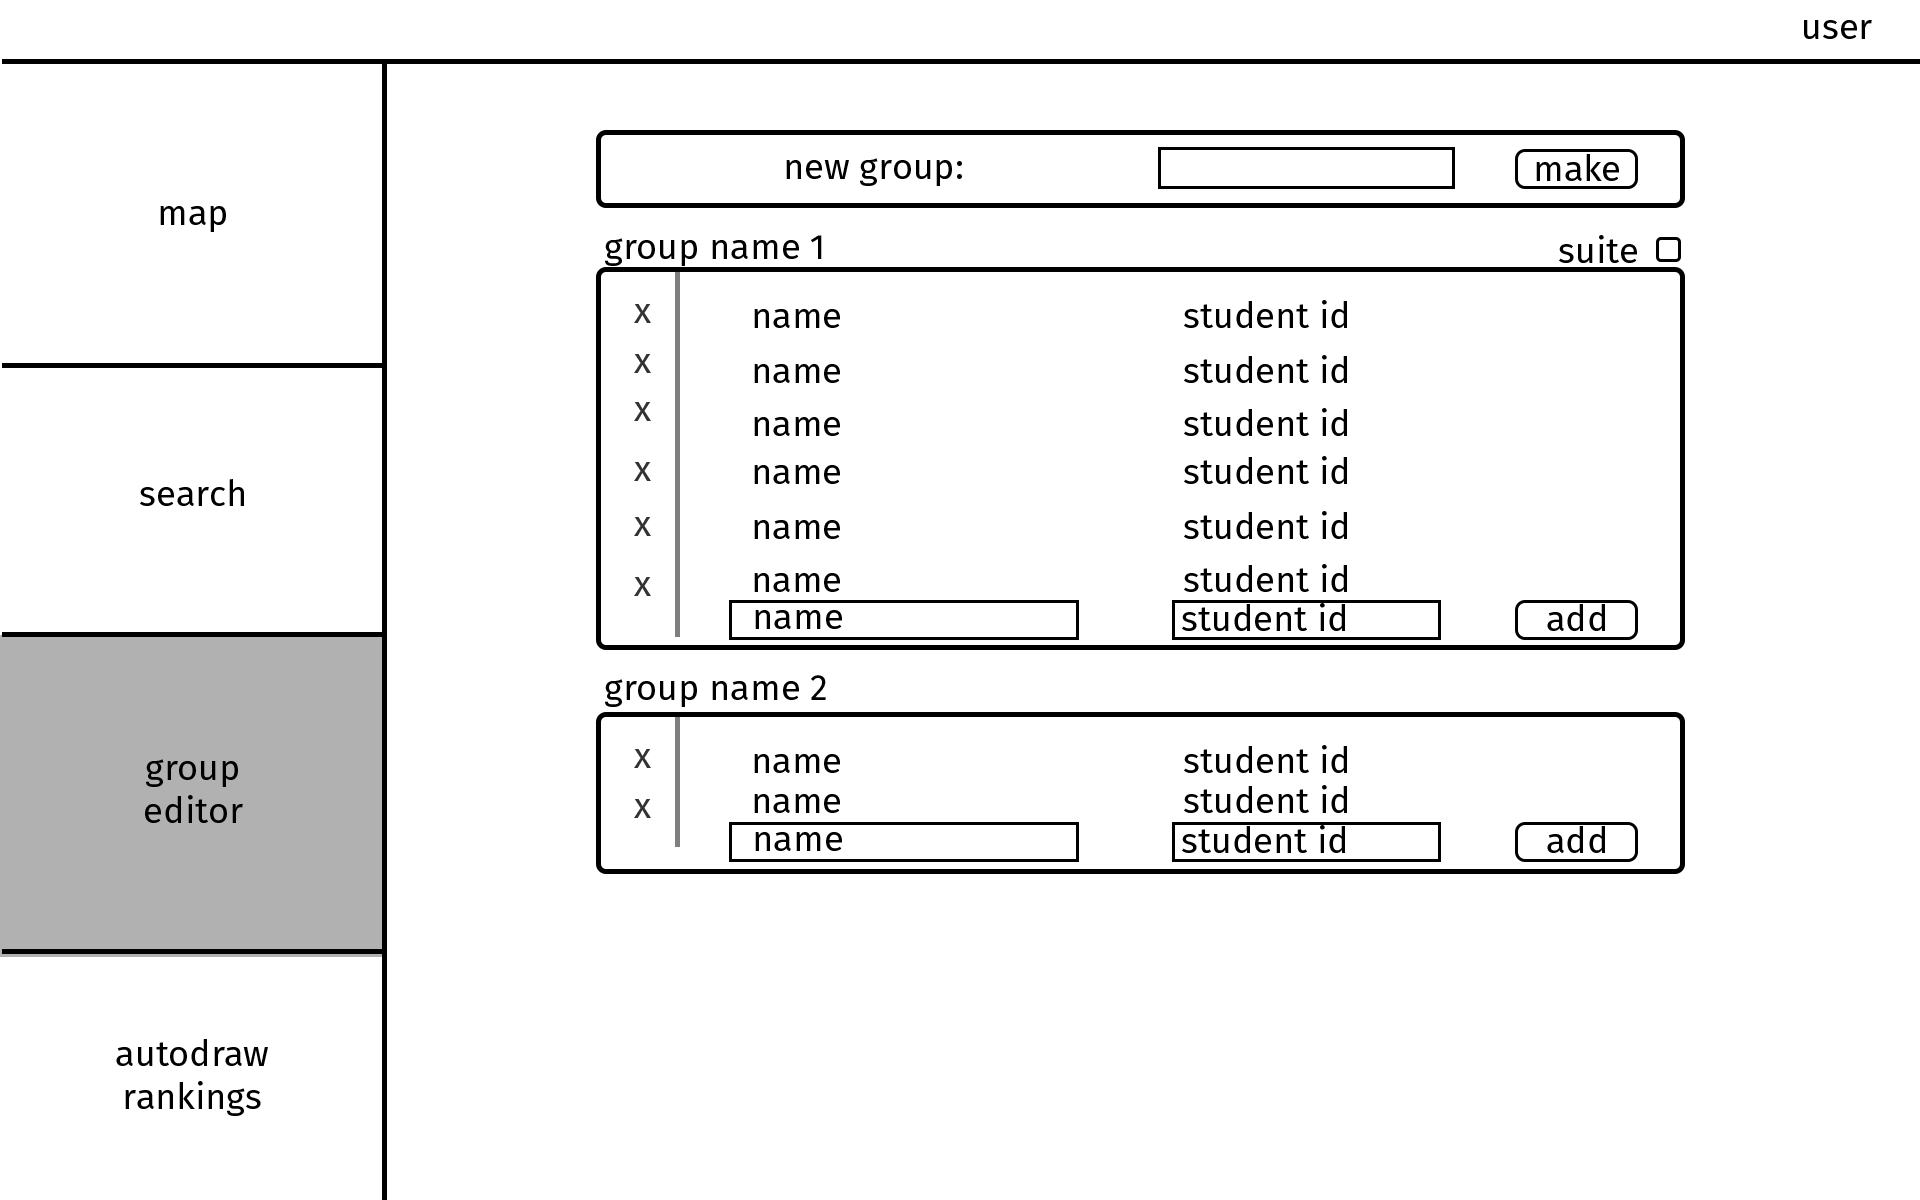
\includegraphics[scale=.15]{wireframe/group}
\caption{a page to manage one's groups}
\label{fig:wiregroup}
\end{figure}

The third choice on the left bar loads the ``Group Editor'' as shown in
\cref{fig:wiregroup}. On this page, one may create a new group, or edit an
existing group. Editing includes adding or removing group members. If a group
has three members, the ``suite'' checkbox may be toggled. Otherwise, the
checkbox is unchecked for groups of two or smaller and is checked for groups
larger than three. A group may have no more than six individuals, and a user is
limiting to participating in at most one suite group.

\subsubsection{Autodraw Preference Page}
\begin{figure} \centering

\includegraphics[scale=.15]{wireframe/autodraw}
\caption{a page to sort one's room collection preferences to automate the
    drawing process}
\label{fig:wireprefs}
\end{figure}

The final choice for a user is the ``Autodraw'' page, shown in
\cref{fig:wireprefs}. On this page, a user designates a ranking for the various
collections previously chosen. Each preference designates a collection and a
group. We imagine these preferences to be draggable, for easy re-ordering. This
page functions so that students need not be available at exactly their draw time
(or time corresponding to their draw number, depending on implementation) and so
that the whole process can to some extent be automated.

A possible extension may be to allow a user to directly add to their queue
without having to go back to the search page.

\subsection{Admin Pages}

In the sections that follow, we briefly describe some additional pages available
to adminstrators. We currently consider these pages to be beyond the scope our
our project currently, but serve as possible extensions.

\subsubsection{Admin Suite Editor}
\begin{figure} \centering
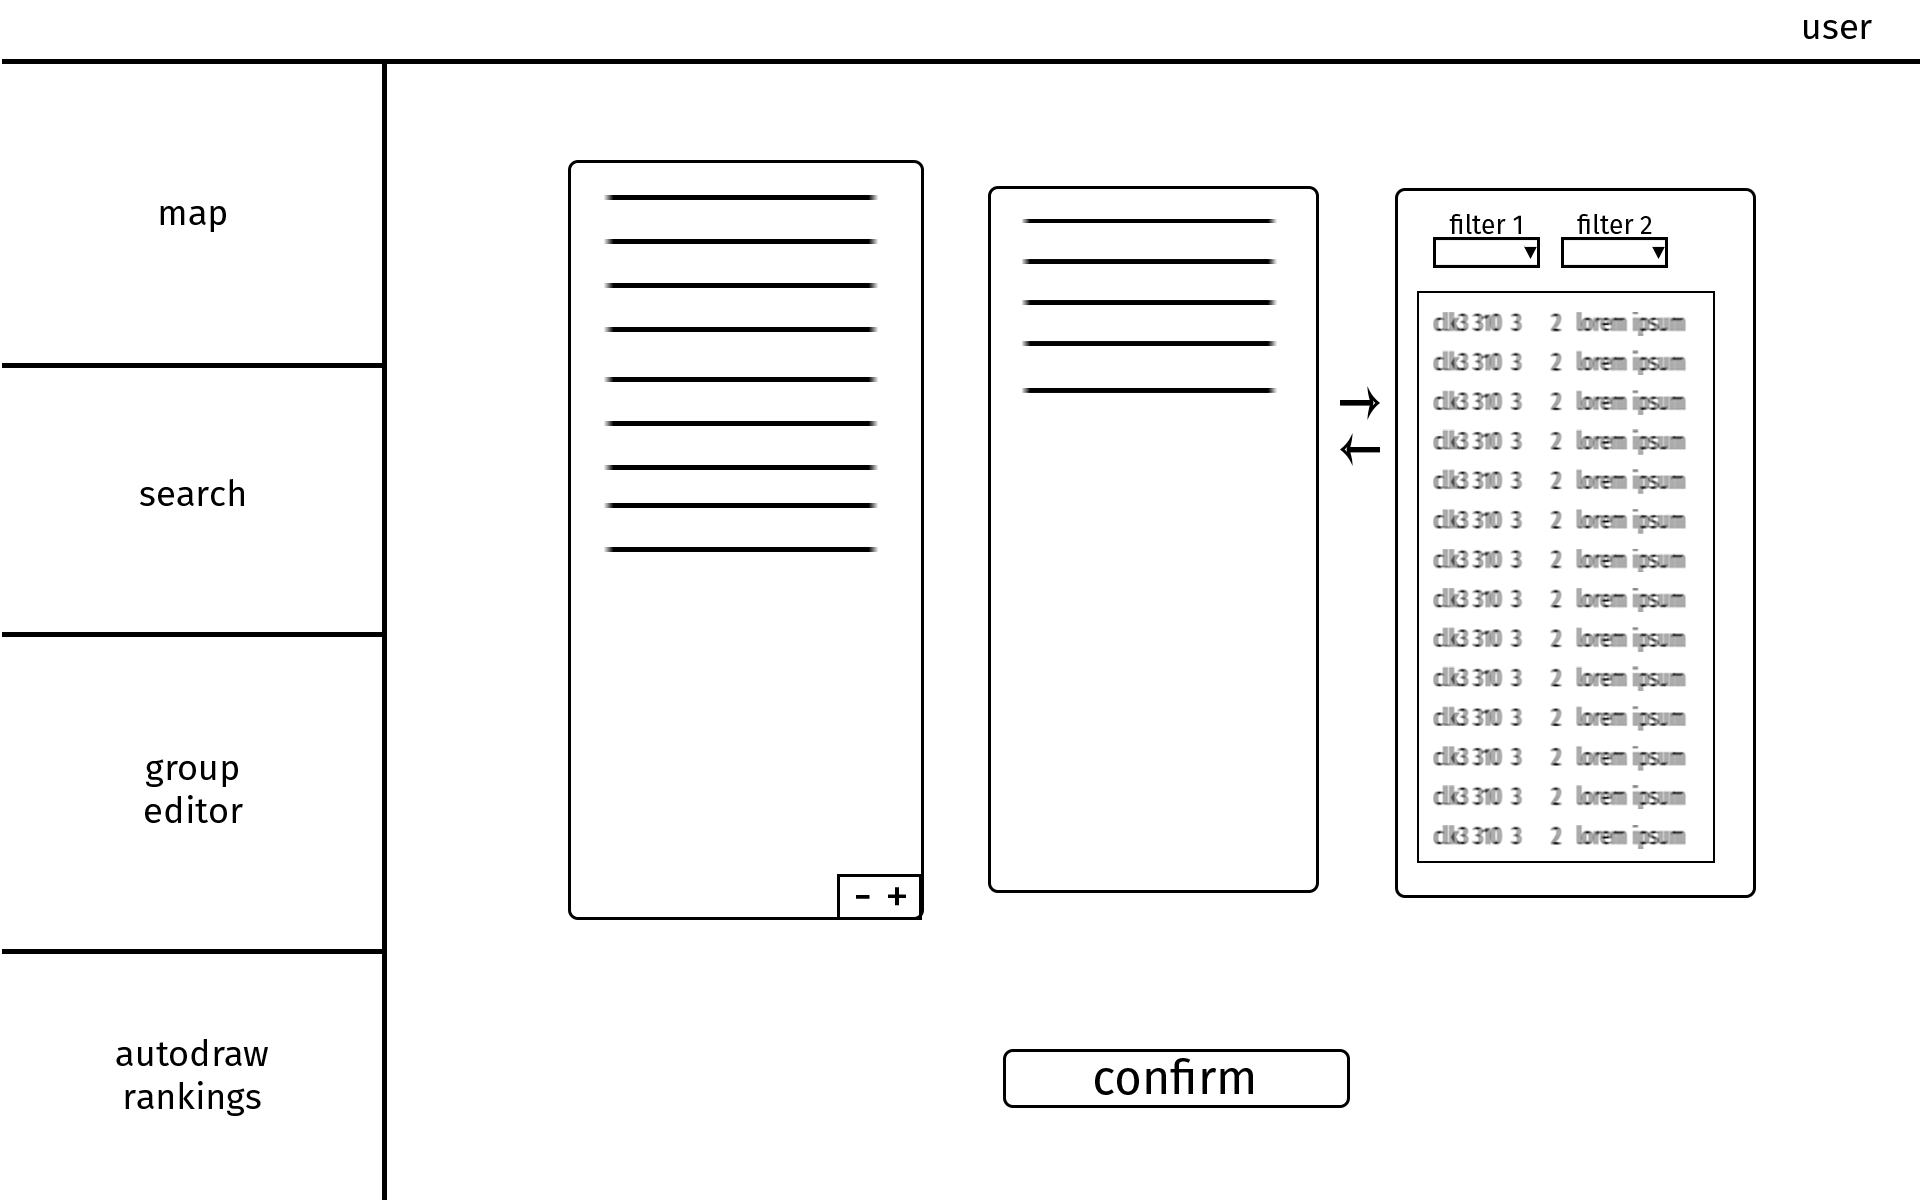
\includegraphics[scale=.15]{wireframe/admin_suite_editor}
\caption{a suite editing page for admins}
\label{fig:wireadmin-suite-editor}
\end{figure}

\Cref{fig:wireadmin-suite-editor} shows what a ``suite-editor'' could look like.
We imagine this page such that it lists existing suites in the leftmost of the
three panes. This pane allows for a suite to be deleted as well as for a new
collection to be designated. The middle pane displays the rooms that make up the
collection. The rightmost pane allows filtering through dorms not yet part of a
collection. Between the middle and right panes are left and right arrows.
Respectively, these arrows allow a room to be added and removed from the
currently selected collection.

\subsubsection{Admin Assignment Editor}
\begin{figure} \centering
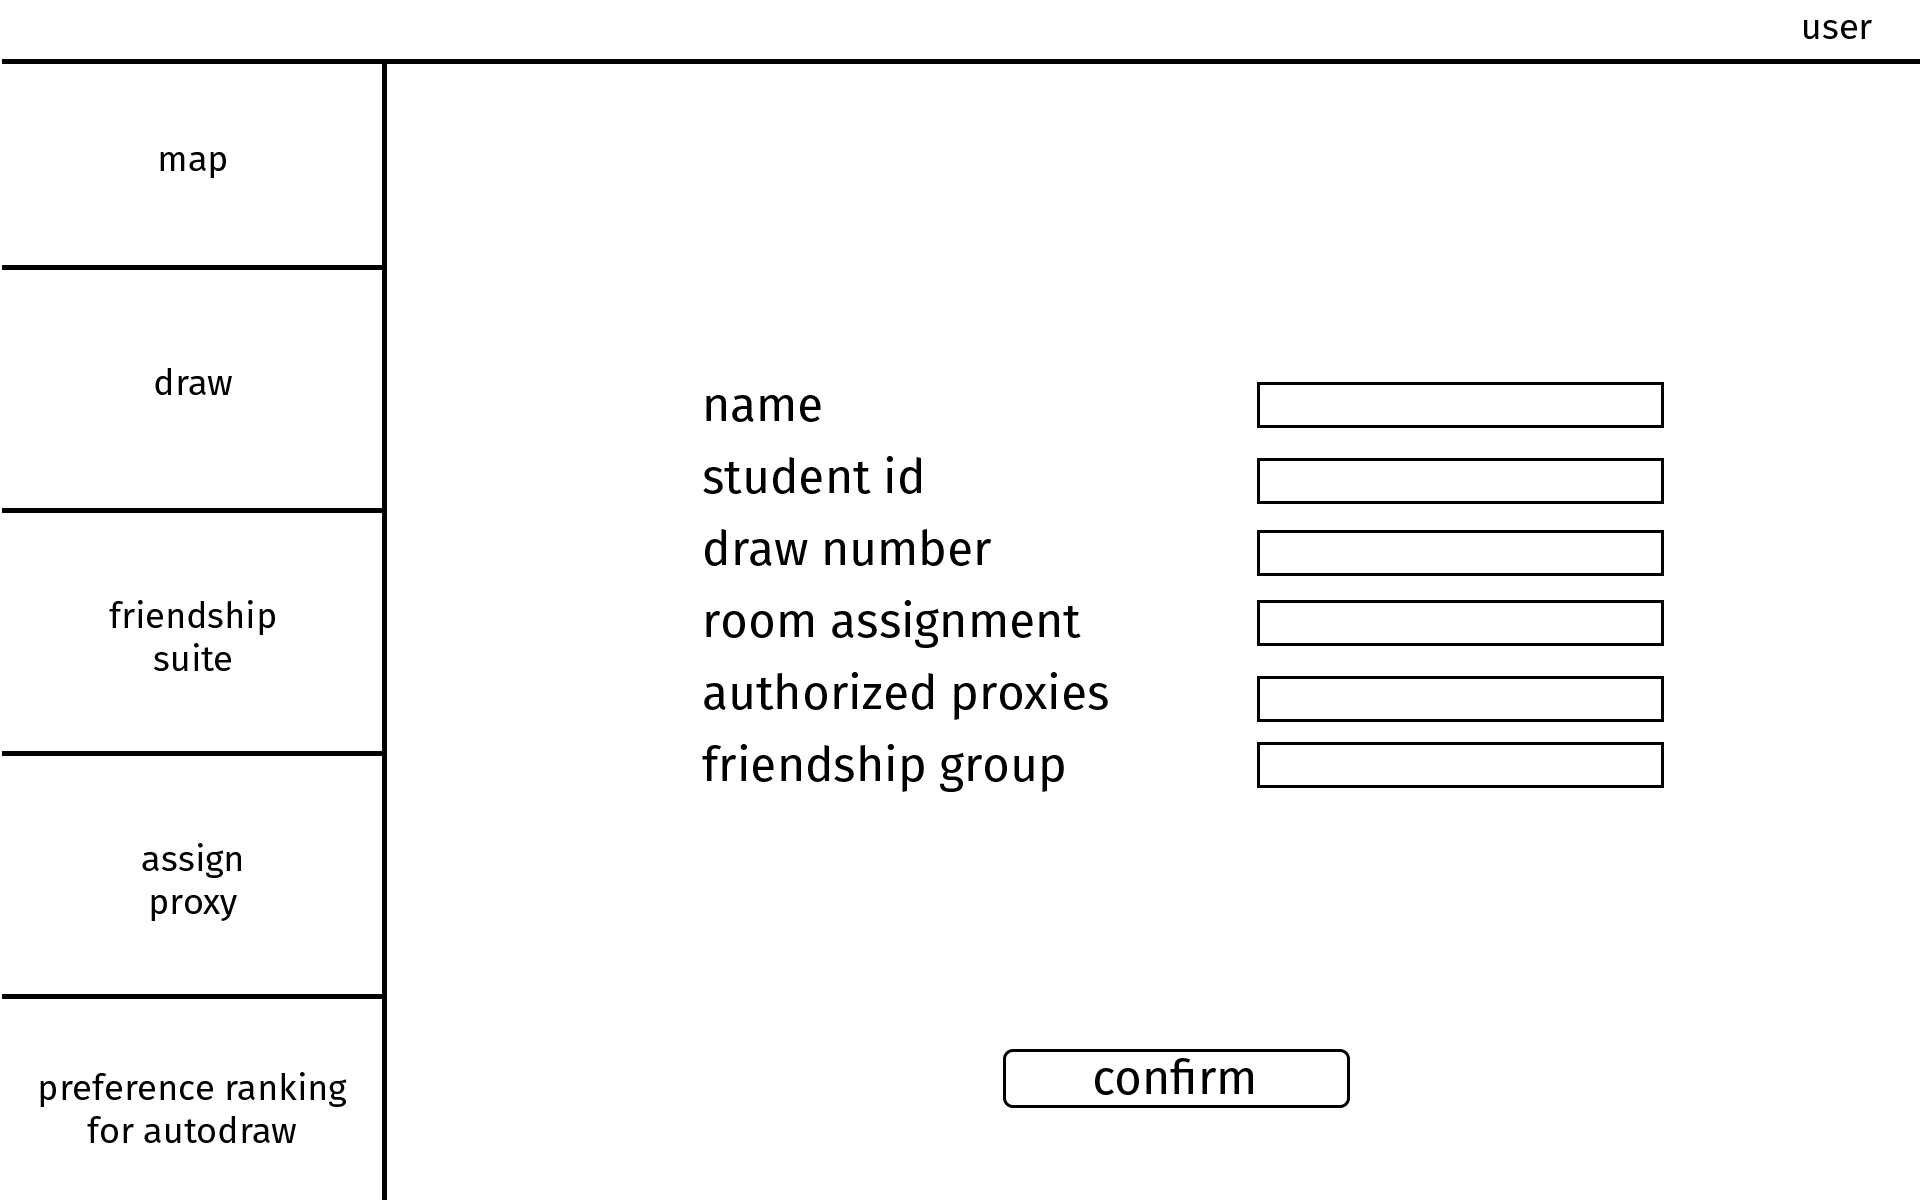
\includegraphics[scale=.15]{wireframe/admin_assignment_editor}
\caption{an assignment editing page for admins}
\label{fig:wireadmin-assignment-editor}

The ``Admin Assignment Editor'' (\cref{fig:wireadmin-assignment-editor}) would
allow an admin to make changes to current assignments. This might include
changing a student's draw number and room to which a student is assigned.
\end{figure}